\chapter{PENGUJIAN}
\label{sec:chap4_pengujian}
\vspace{1ex}

\section{Pengujian Integrasi Sistem secara Keseluruhan}
Pengujian sistem dilakukan dengan menguji interaksi seluruh komponen yang telah diintegrasikan, meliputi antarmuka pengguna web Next.js, server FastAPI klien Model Context Protocol, server FastMCP lokal pada robot, serta tumpukan navigasi Robot Operating System. Pengujian dilakukan dalam skenario operasional inspeksi visual pada area dalam ruangan secara langsung. Operator mengirimkan perintah dalam bahasa alami untuk menginstruksikan robot melakukan pemeriksaan terhadap beberapa objek target di lantai tertentu. Sesi pengujian dimulai dengan inisialisasi sesi pada antarmuka web, diikuti oleh pencarian dokumen prosedur standar, perencanaan rute kunjungan objek, navigasi fisik robot ke lokasi target, hingga pengambilan serta analisis \textit{image} target berdasarkan dokumen prosedur standar yang relevan.

Berdasarkan hasil pengujian secara menyeluruh yang telah dilakukan, sistem secara umum mampu menjalankan alur inspeksi visual otonom dengan baik, namun masih ditemukan beberapa kendala operasional. Kendala pertama terjadi pada sistem navigasi robot, di mana robot sesekali membatalkan perintah navigasi karena gagal menemukan jalur alternatif saat berada sangat dekat dengan rintangan fisik di dalam ruangan. Hal ini disebabkan oleh konfigurasi batas jarak aman pembacaan sensor serta parameter toleransi tabrakan pada perencana jalur lokal yang terlalu sensitif. Kendala kedua ditemukan pada hasil analisis visual oleh model bahasa besar multimodal Google Gemini, di mana model mampu melakukan evaluasi dengan akurat untuk instruksi prosedur standar yang bersifat sederhana dan objektif seperti memeriksa keberadaan objek, posisi tegak objek, atau kesesuaian warna objek. Namun, untuk instruksi prosedur standar yang bersifat abstrak seperti memeriksa apakah ujung selang menempel dengan benar pada badan alat pemadam api ringan, model terkadang memberikan hasil analisis yang kurang konsisten. Kendala ketiga berkaitan dengan pemotongan \textit{image} otomatis di mana koordinat pembatas objek yang diprediksi oleh model bahasa besar mengalami sedikit pergeseran dari posisi objek sebenarnya, sehingga \textit{image} hasil pemotongan oleh pustaka OpenCV terlihat kurang presisi di galeri antarmuka web, meskipun kesalahan pemotongan ini tidak memengaruhi hasil analisis akhir karena model tetap menerima berkas \textit{image} asli secara penuh.

\begin{figure}[h!]
    \centering
    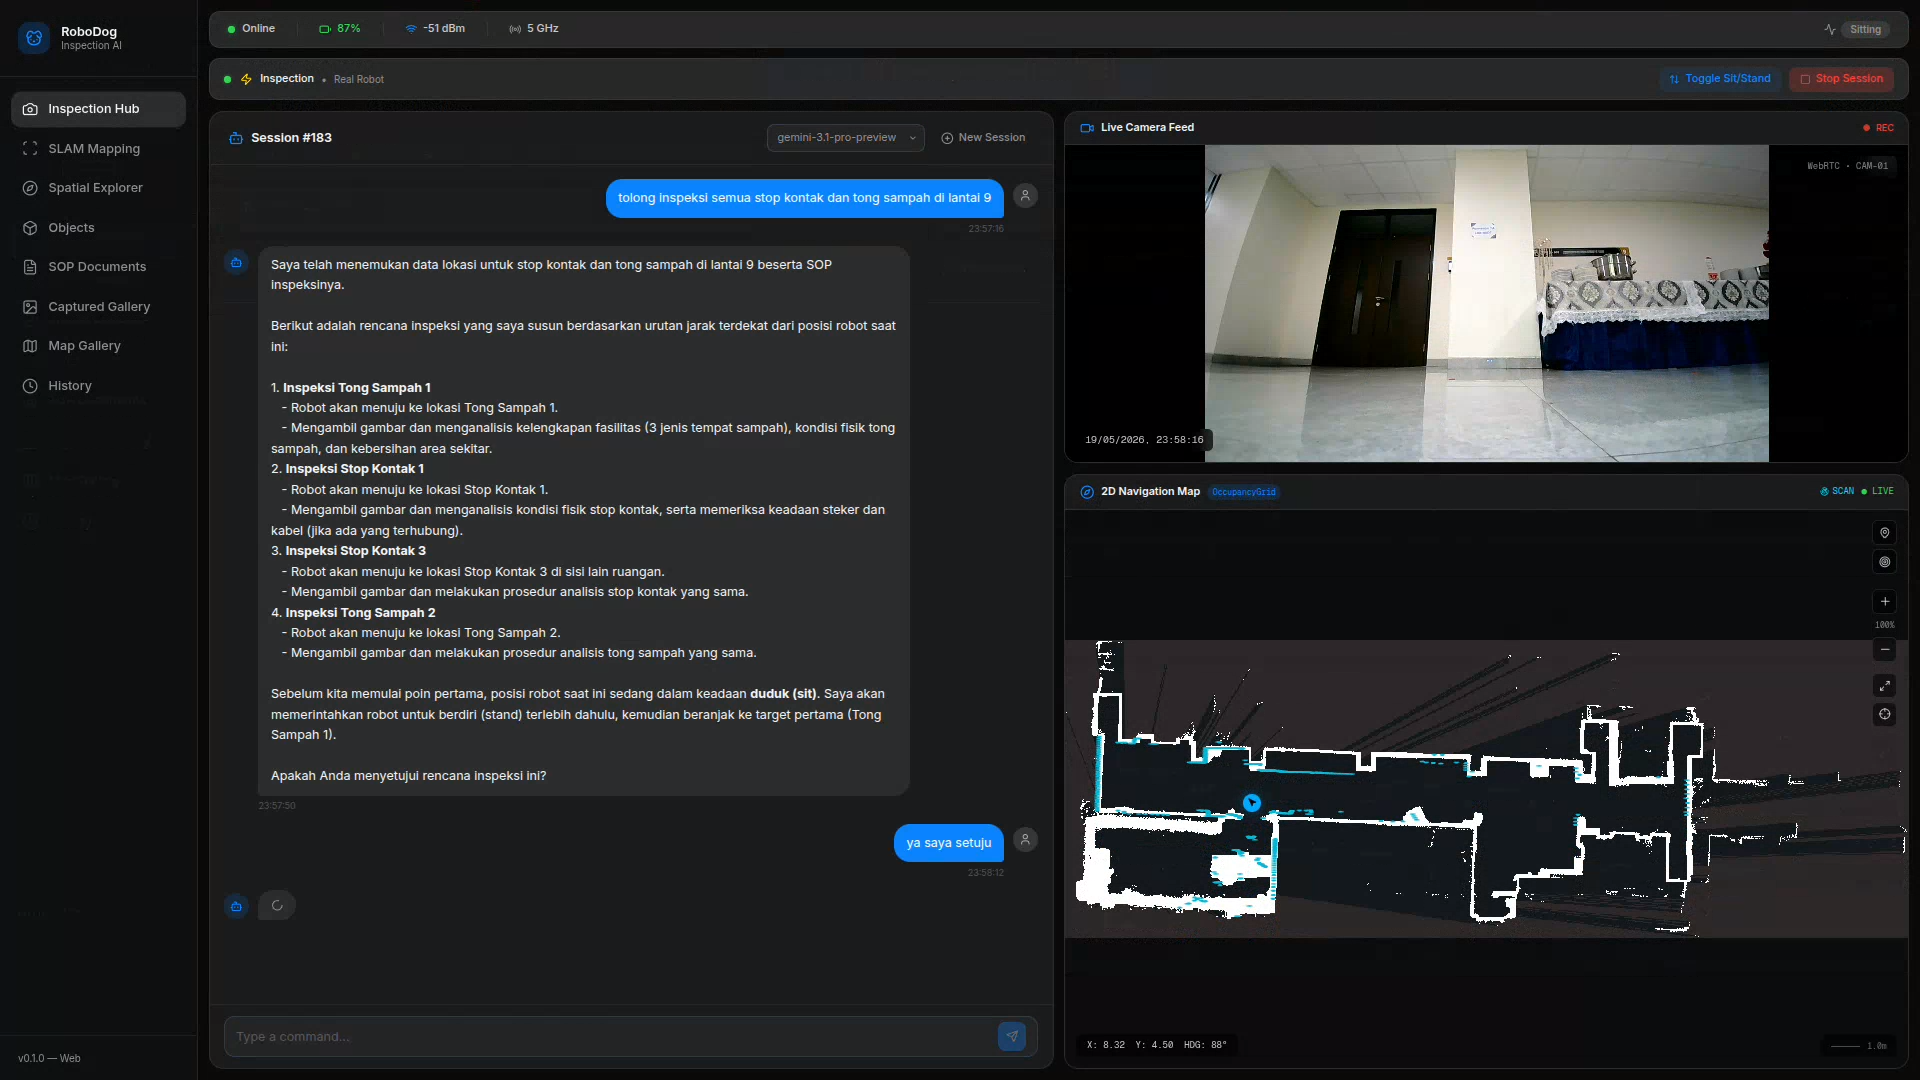
\includegraphics[width=0.8\textwidth]{Init/gambar/planning.png}
    \caption{Tampilan Proses Planning}
    \label{fig:planning}
\footnotesize \textbf{Sumber:} Dokumentasi Penulis
\end{figure}

\begin{figure}[h!]
    \centering
    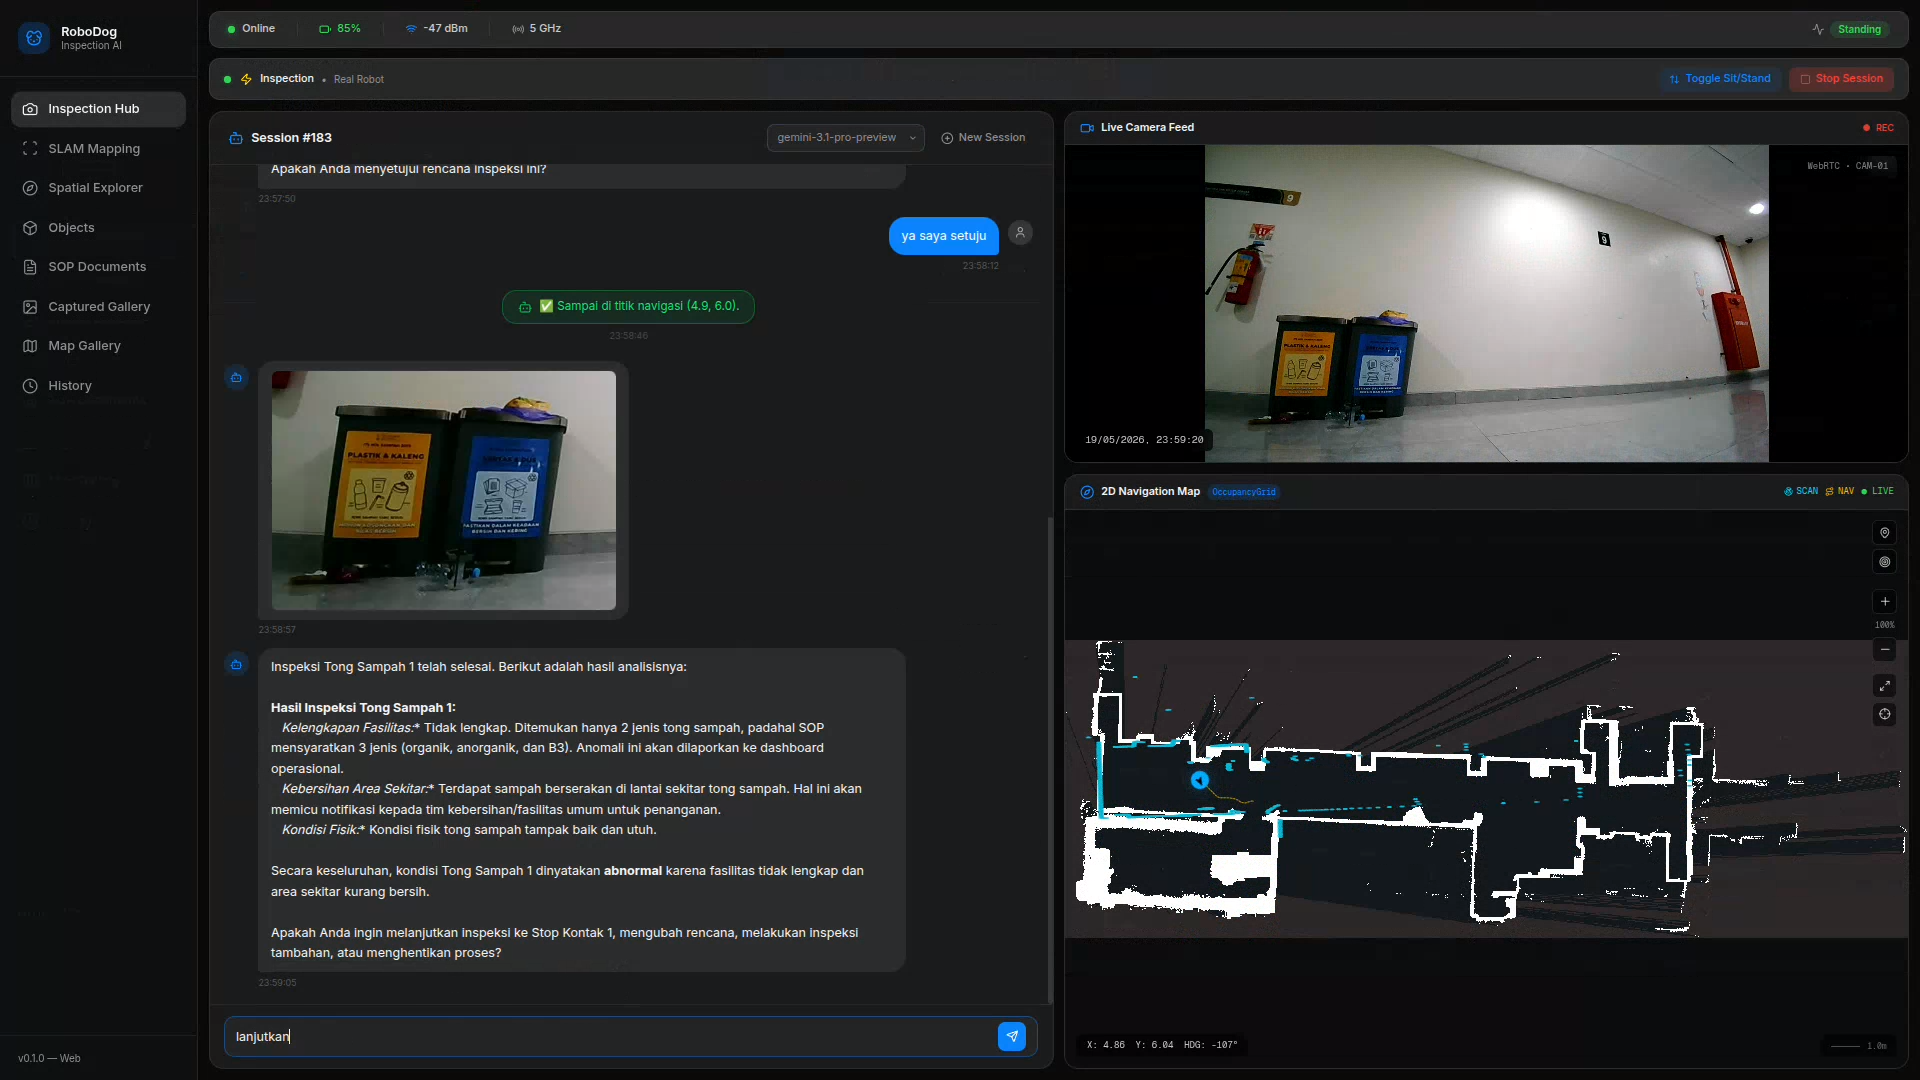
\includegraphics[width=0.8\textwidth]{Init/gambar/inspection_result.png}
    \caption{Tampilan Hasil Inspeksi}
    \label{fig:inspection_result}
\footnotesize \textbf{Sumber:} Dokumentasi Penulis
\end{figure}

\section{Analisis Latensi dan Konsumsi Token}
\begin{figure}[h!]
    \centering
    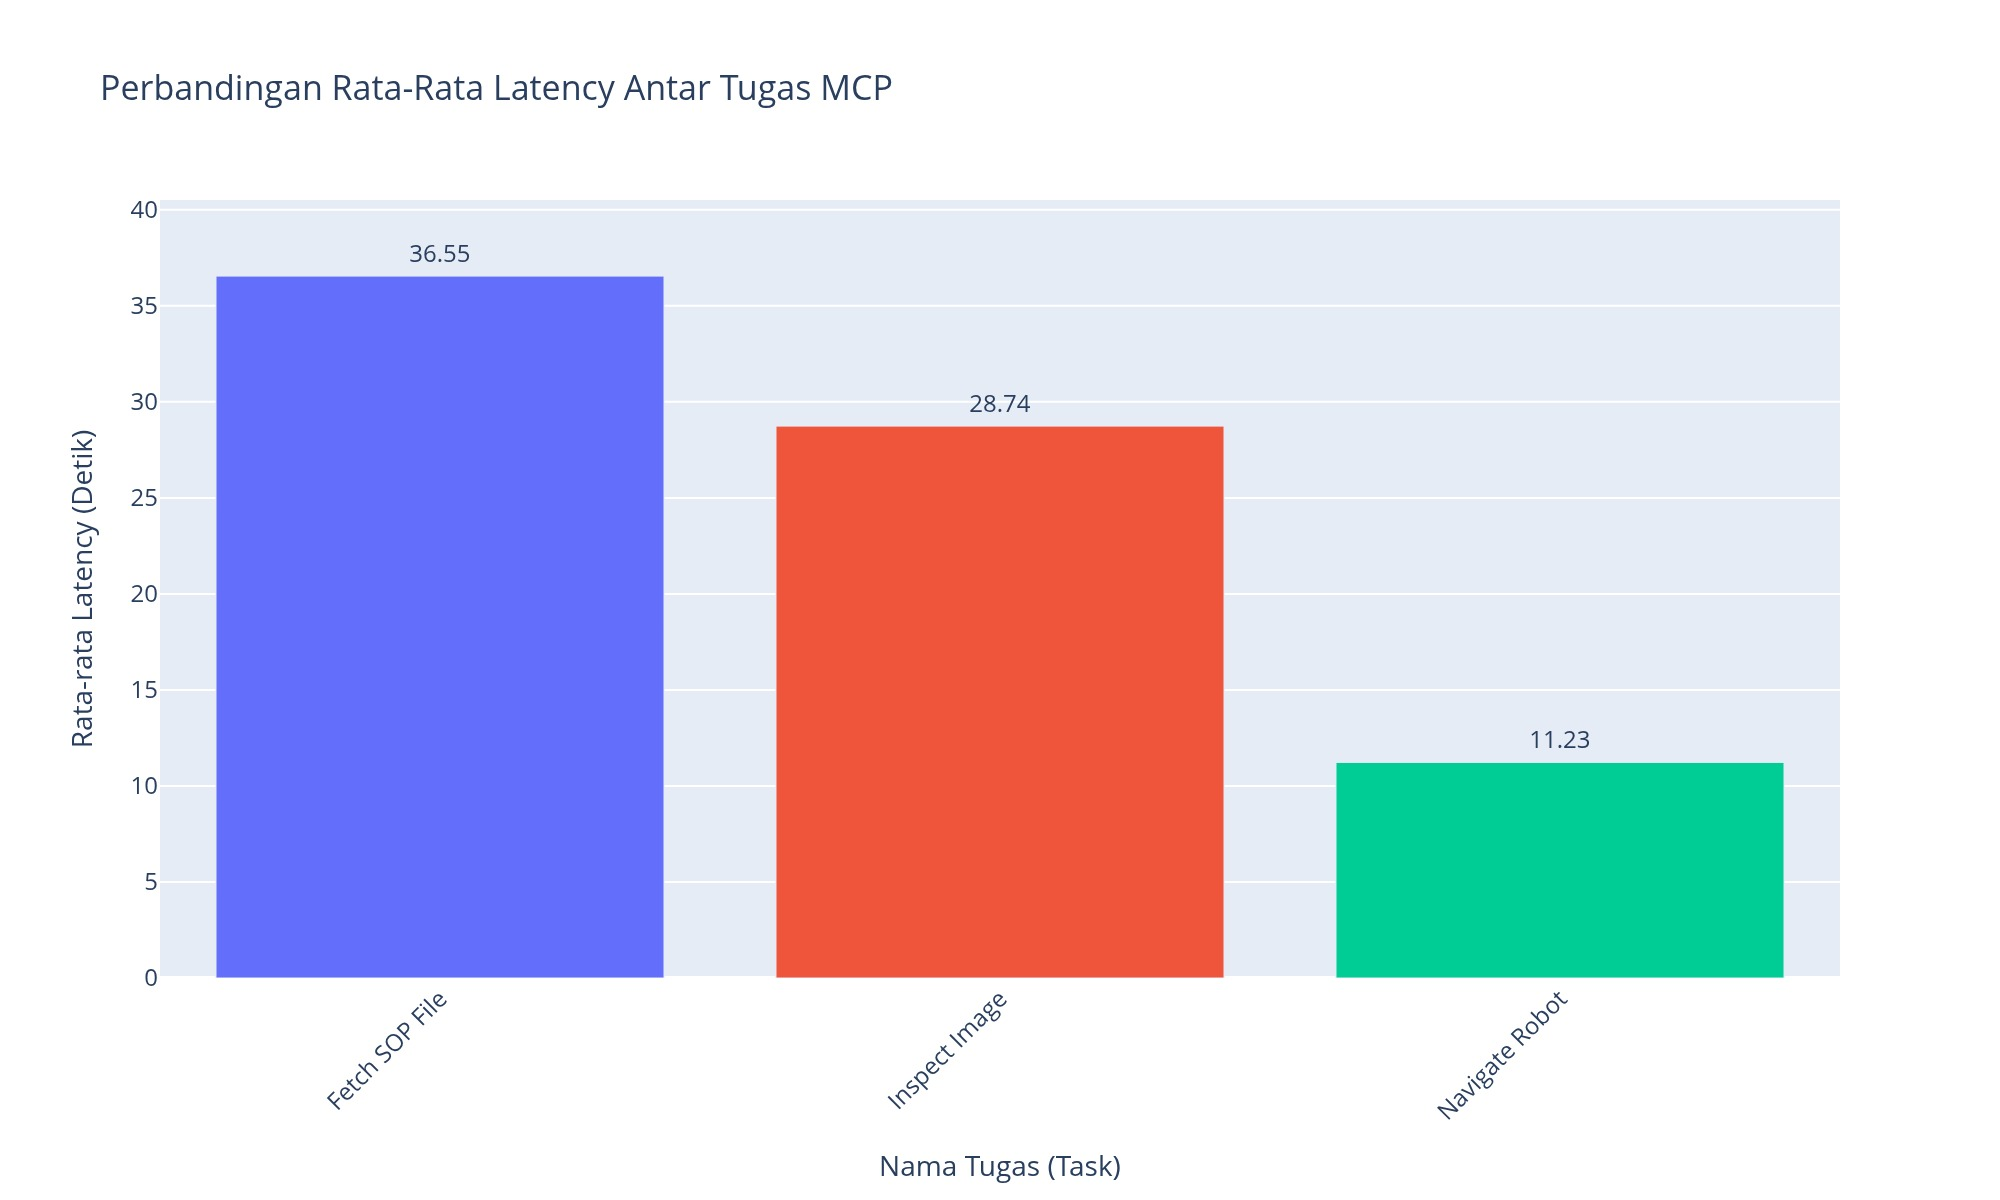
\includegraphics[width=0.8\textwidth]{Init/gambar/latency_mcp_comparison.jpg}
    \caption{Perbandingan Rata-Rata Latensi Antar Tugas Model Context Protocol}
    \label{fig:latency_mcp_comparison}
\footnotesize \textbf{Sumber:} Dokumentasi Penulis
\end{figure}

\begin{figure}[h!]
    \centering
    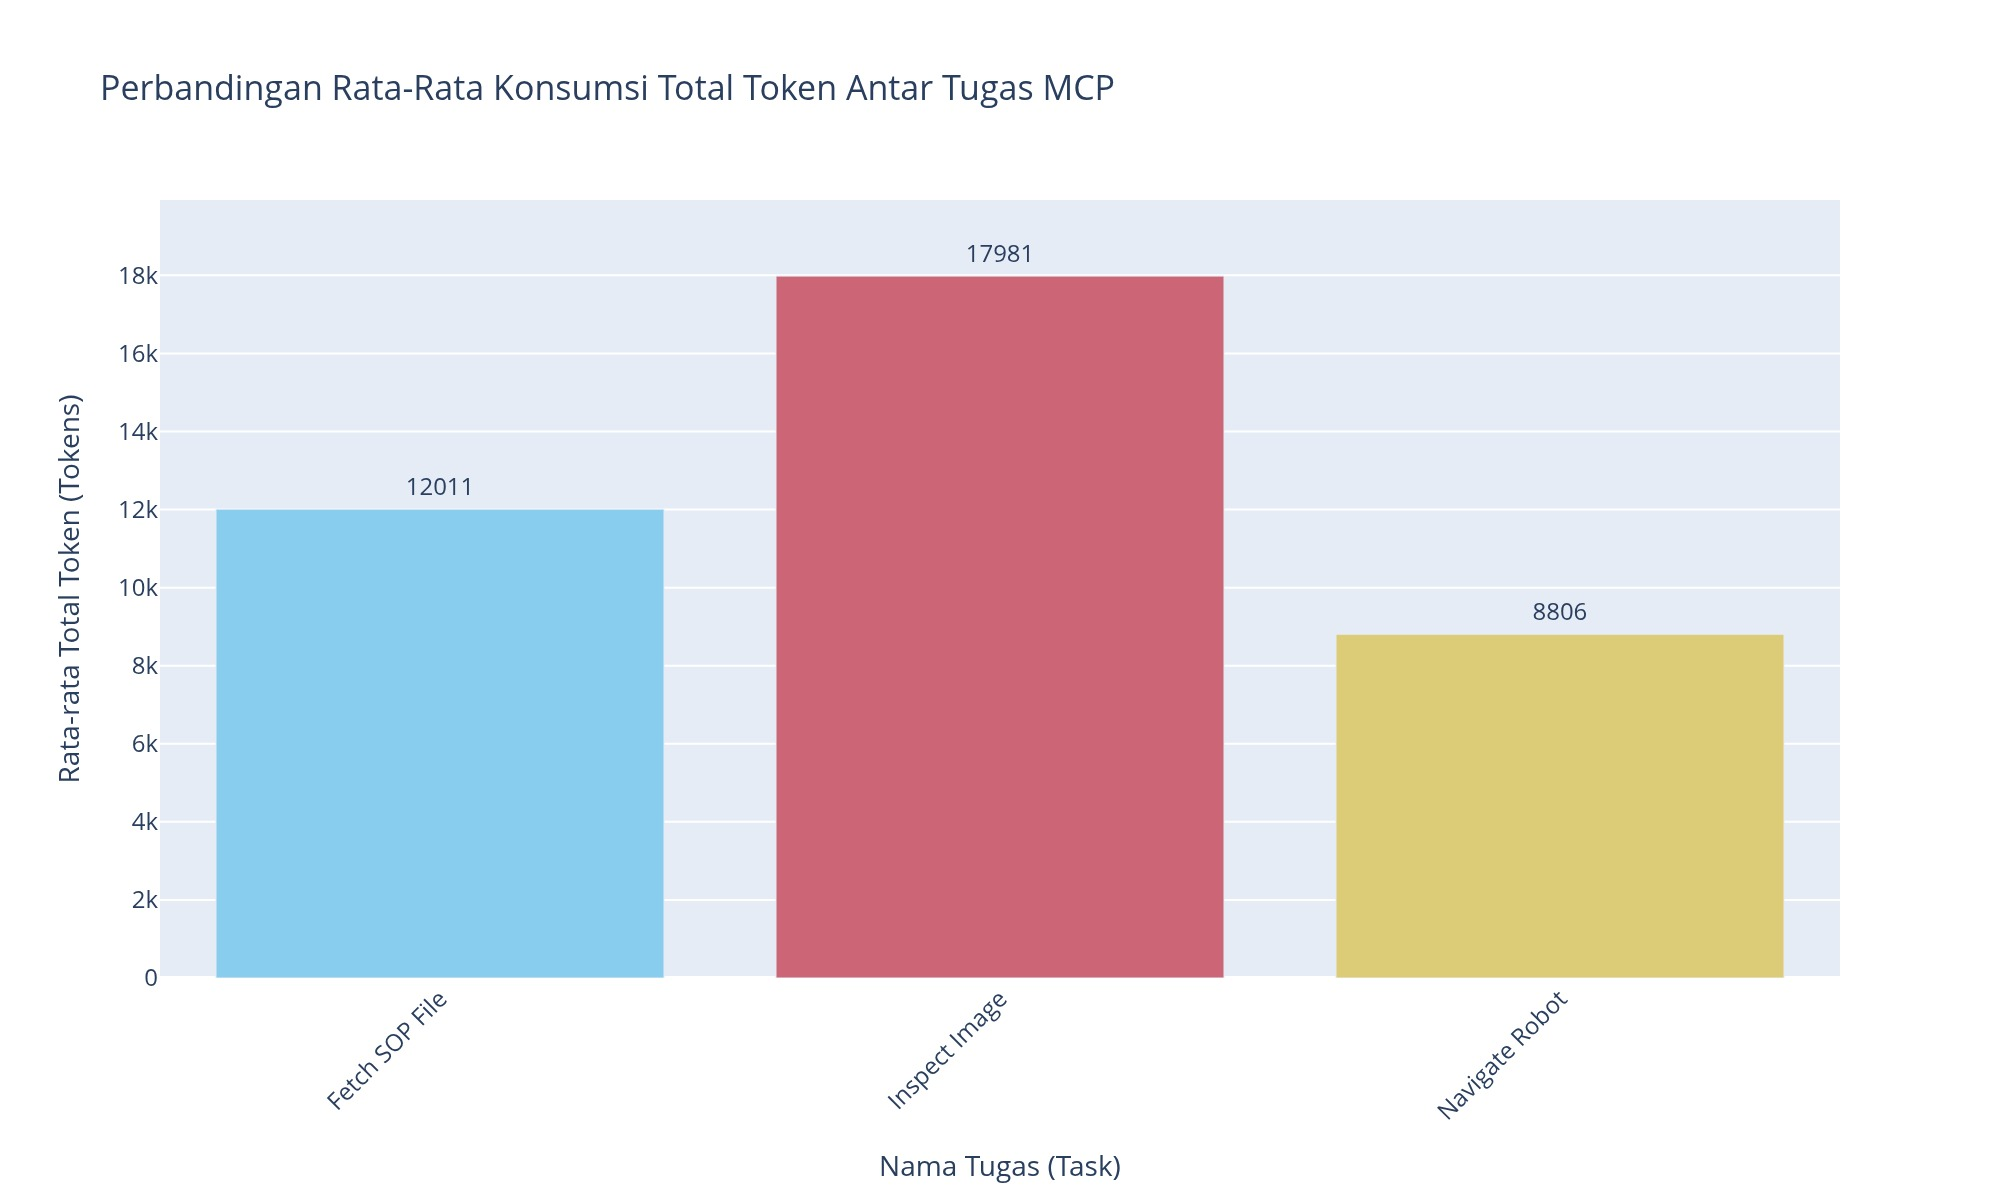
\includegraphics[width=0.8\textwidth]{Init/gambar/tokens_mcp_comparison.jpg}
    \caption{Perbandingan Rata-Rata Konsumsi Token Antar Tugas Model Context Protocol}
    \label{fig:tokens_mcp_comparison}
\footnotesize \textbf{Sumber:} Dokumentasi Penulis
\end{figure}

Selain pengujian fungsional secara keseluruhan, dilakukan pula analisis terhadap kinerja sistem berdasarkan parameter waktu tunggu atau latensi serta konsumsi token model bahasa besar. Data pengujian ini diekstraksi dari riwayat pencatatan aktivitas sistem pemantauan Langfuse selama proses uji coba pengembangan sistem dilakukan, sehingga data yang digunakan mencerminkan performa nyata dari berbagai variasi interaksi pengguna tanpa manipulasi lingkungan pengujian. Parameter evaluasi difokuskan pada tiga jenis tugas utama yang dijalankan oleh agen kecerdasan buatan melalui pemanggilan alat Model Context Protocol, yaitu tugas pengambilan berkas prosedur standar, tugas pengambilan dan analisis \textit{image}, serta tugas navigasi robot.

Hasil pengukuran rata-rata latensi untuk masing-masing tugas ditunjukkan pada Gambar \ref{fig:latency_mcp_comparison}. Tugas pengambilan berkas prosedur standar memiliki rata-rata latensi tertinggi yaitu sekitar 36,55 detik. Waktu tunggu yang lama ini disebabkan oleh kebutuhan sistem untuk mengunduh dokumen panduan inspeksi dari penyimpanan Supabase, memproses teks di dalamnya, dan mengirimkannya kembali untuk dianalisis oleh model bahasa besar. Tugas pengambilan dan analisis \textit{image} membutuhkan waktu rata-rata sekitar 28,74 detik, yang dipengaruhi oleh durasi pengambilan foto dari kamera robot, pemrosesan citra dengan OpenCV, pengunggahan hasil foto ke penyimpanan Supabase, serta evaluasi visual multimodal oleh model Gemini. Sementara itu, tugas navigasi robot menunjukkan rata-rata latensi sekitar 11,23 detik, yang mencerminkan durasi pengiriman perintah koordinat secara asinkron hingga sistem navigasi utama memproses instruksi tersebut.

Hasil analisis konsumsi rata-rata token untuk setiap tugas ditunjukkan pada Gambar \ref{fig:tokens_mcp_comparison}. Tugas pengambilan dan analisis \textit{image} mengonsumsi token rata-rata tertinggi yaitu sekitar 17980 token karena model harus memproses informasi visual berupa berkas \textit{image} beresolusi tinggi yang membutuhkan representasi token multimodal yang sangat besar. Tugas pengambilan berkas prosedur standar mencatatkan konsumsi rata-rata sekitar 12010 token, yang didominasi oleh jumlah teks panduan inspeksi yang dibaca ke dalam memori kerja model. Tugas navigasi robot membutuhkan rata-rata konsumsi terendah yaitu sekitar 8806 token, karena perintah navigasi hanya melibatkan pertukaran informasi koordinat numerik serta status posisi robot yang relatif sederhana.
